\chapter{Réalisation}
%Tout doit être au présent

Dans l'optique de détecter toutes les variations somatiques des TFBS dans les LMS, j'utilise les logiciels \textbf{Mutect} et \textbf{Varscan}. L'utilisation de \textbf{Mutect} nécessite une organisation spécifique des données. J'utilise plusieurs outils pour formater les fichiers d'alignement suivant les exigences de celui-ci. Tous ces outils sont intégrés à un pipeline d'analyse développé en bash qui nécessite de nombreuses ressources en mémoire pour fonctionner de façon optimale.

L'équipe \textit{Génétique et biologie des sarcomes} de l'institut Bergonié travaille en collaboration avec le \textit{\acrlong{mcia}} (\acrshort{mcia}) \citep{MCIA} qui met à disposition de ses utilisateurs un serveur de calcul constitué de 264 noeuds de calculs ayant 48 Gb de mémoire chacun, 4 noeuds de calcul avec 512Gb de mémoire et 2 noeuds pour les outils de visualisation.

Les données issues de techniques de séquençage NGS de génomes complets étant très volumineuses (voir la partie \ref{subsec:NGS}), je dois optimiser le temps d'exécution de mon pipeline. J'utilise donc les ressources du \textit{MCIA} mises à ma disposition.

\section{Organisation des données}

Le but de mon projet est de rechercher les variations somatiques touchant les TFBS. La première étape de mon pipeline d'analyse est donc l'extraction des séquences chevauchant les TFBS dans les fichiers d'alignements.

J'utilise un des outil du logiciel \textbf{Samtools} et une base de données contenant les positions des TFBS pour extraire toutes les séquences chevauchantes. L'extraction réalisée, produit un fichier dont la taille est réduite de 90\%. Lors de l'extraction, \textbf{Samtools} récupère toutes les séquences qui chevauchent la séquence d'intérêt d'au moins une paire de base. Les séquences contenues dans le fichier d'alignement mesurent au maximum 101bp, lorsqu'une base est commune entre la séquence et la région du TFBS, la séquence est récupérée par le logiciel. Ainsi les séquences récupérées peuvent couvrir jusqu'à 100 pb de plus à gauche et 100 pb de plus à droite que la région d'intérêt comme l'illustre la figure \ref{fig:sequence}.

\begin{figure}[h]
\centering
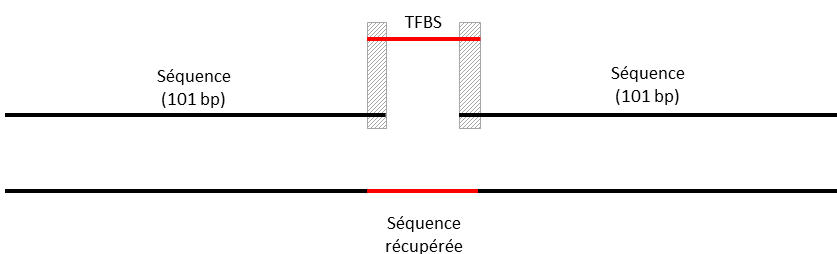
\includegraphics[scale=0.5]{Figures/sequence.png}
\caption{Fonctionnement de \textbf{Samtools}}
\label{fig:sequence}
\end{figure}

Pour utiliser les outils de \textbf{GATK} nécessaires à la détection de variants somatiques, un trie caryotypique des séquences contenues dans les fichiers d'alignement et un ajout des \og read group\fg ~est indispensable. J'utilise les outils \textit{\textbf{AddOrReplaceReadGroup}} et \textit{\textbf{ReorderSam}} du logiciel \textbf{Picardtools} pour trier et respectivement ajouter la nomenclature, selon les exigences de \textbf{GATK}. L'utilisation de \textit{\textbf{ReorderSam}} implique que le fichier d'entrée soit trié suivant les coordonnées de chaque séquence. J'utilise donc le paramètre \textit{\textbf{SORT\_ORDER}} de \textit{\textbf{AddOrReplaceReadGroup}} afin d'obtenir des fichiers convenablement triés.

Les fichiers d'entrées de \textbf{GATK} doivent être indexés, j'utilise un outil de \textbf{Samtools} pour répondre à cette exigence.

Les fichiers d'alignement présentent généralement des erreurs liées au séquençage et à l'alignement. Dans le but de limiter le nombre de faux positifs liés à ces erreurs, j'utilise plusieurs outils de \textbf{GATK}. Ces outils me permettent de ré-aligner localement les bases et de les recalibrer. Toutes les bases qui ne se sont pas ré-alignées sur le génome de référence et qui présentent plus d'un pourcent de \og mismatch\fg ~sont éliminées. Les fichiers ainsi obtenus sont passés en paramètre d'entrée aux logiciels de détection de variants somatiques.

\section{Détection des variants somatiques}

Afin de détecter les variants somatiques, j'utilise deux logiciels différents, \textbf{MuTect} et \textbf{Varscan}, sélectionnés d'après les critères expliqués dans la partie \ref{sec:detec}. 

Face au nombre important d'échantillons à traiter (148), j'utilise l'outil de parallélisation de \textbf{GATK}, \textit{\textbf{Queue}}, pour exécuter \textbf{MuTect}, et un nœud de calcul de 48G complet. J'ai écrit un script en Scala qui découpe les fichiers d'alignements suivant une limite fixée par un paramètre d'entrée et exécute \textbf{MuTect} pour chacun des fragments. Une fois tous les fragments traités, ce script les assemble en un seul fichier de sortie au format VCF.

Lors de l'exécution des outils de détection je ne veux récupérer que les variations somatiques n'ayant jamais été observées. Un des paramètres d'entrée de \textbf{MuTect} permet de filtrer suivant les positions indiquées dans un fichier. Je donne le fichier VCF de 1000G de façon à ce que toutes les variations détectées et présentes dans ce fichier soient éliminées du fichier de sortie. Je ne veux également conserver que les variations couvertes par 14 séquences au minimum dans le fichier de tumeur et 8 dans le fichier constitutionnel, \textbf{MuTect} est donc paramétré selon ces critères. Un dernier filtre me permet d'isoler les variations pour lesquelles la fréquence allélique est d'au minimum 30\%.

J'utilise le logiciel \textbf{Varscan} en complément de \textbf{MuTect} pour identifier les variations somatiques des TFBS. Il n'est pas possible de donner une base de données à ce logiciel, pour filtrer les variants, en revanche, il est possible de paramétrer la couverture de séquençage. Je donne donc en entrée les couvertures minimales souhaitées pour les échantillons constitutionnels et tumoraux. Je paramètre également \textbf{Varscan} pour qu'il produise un fichier VCF en sortie contenant des variants ayant tous une fréquence allélique de 30\% minimum.

Pour obtenir les variations somatiques les plus probables, je réalise une  intersection des deux fichiers VCF obtenus en sortie de \textbf{MuTect} et \textbf{Varscan}. Le fichier obtenu contient les variants somatiques détectés dans toutes les séquences des fichiers d'entrée, certains ne concernent donc pas les TFBS ce qui ne perturbe pas la suite de l'analyse, à savoir l'annotation.

\newpage
\section{Annotation des variants somatiques}

Afin de documenter le plus précisément possible les variants somatiques que je détecte, j'utilise le logiciel \textbf{Annovar} et la base de données \textit{\textbf{tfbsConsSites}}.

Dans un script écrit en bash, je transforme les fichiers VCF issus des logiciels de détection de variants en fichiers au format avinput qui est propre à \textbf{Annovar}. Je lance ensuite l'annotation en donnant le fichier avinput contenant les variants et la base de données en paramètres d'entrées.  

J'obtiens un fichier annoté pour chacun des échantillons, il contient le nom du TFBS portant la variation, sa localisation ainsi que l'allèle de référence et l'allèle variant. J'analyse ensuite ces fichiers de façon à trouver des éléments communs entre les différents cas du projet.

Le temps d'exécution du pipeline est très important étant donné l'important volume de données à traiter. J'ai pu tester mon pipeline avec différentes options de parallélisation sur les échantillons constitutionnels (C30X et C50X) et tumoraux (T50X et T200X). Les résultats, de ces tests pour les étapes d'organisation des données et de détection des variants sont présentés dans le tableau \ref{tab:time}. 

\begin{table}[h]
\centering
\begin{tabular}{|c|c|c|c|c|c|c|c|c|}
\cline{2-9} \multicolumn{1}{c|}{} & \multicolumn{2}{c|} {C30X} & \multicolumn{2}{c|}{C50X} & \multicolumn{2}{c|}{T50X} & \multicolumn{2}{c|}{T200X} \\
\cline{2-9} \multicolumn{1}{c|}{} & a & b & a & b & a & b & a & b \\
\hline
Read groups & 90 & 15 &  & 30 & 180 & 30 &  & 120 \\
\hline
Réordonner & 120 & 15 &  & 135 & 195 & 30 &  & 135  \\
\hline
Indexation & 5 &  & 15 &  & 5 &  & 15 &  \\
\hline
Ré-aligner & 1200 & 90 &  & 120 & 1800 & 150 &  & 210 \\
\hline
Re-calibrer & 2400 & 210 &  & 270 & 3600 & 300 &  & 625 \\
\hline
MuTect & 1140 & 90 & 1440 & 150 & 2700 & 120 & 3600 & 240 \\
\hline
Varscan & 120 &  & 360 &  & 1020 &  & 1920 &  \\
\hline
\end{tabular}
\captionsetup{justification=centering}
\caption{Récapitulatif des temps d'exécution en minutes\\
\textit{a : sans parallélisation, b : avec parallélisation}}
\label{tab:time}
\end{table}

Pour chacune des étapes, le temps d'exécution est plus important pour les échantillons tumoraux et constitutionnels séquencés à une plus grande profondeur.  

L'ajout des options de parallélisation a pour but d'optimiser le temps de calcul du pipeline et ainsi de traiter le plus rapidement possible chaque échantillon. Les résultats démontrent que les paramètres ajoutés lors du lancement du pipeline en améliorent le temps d'exécution. Tous les échantillons ont ainsi pu être traités au cours de mon stage.

\section{Analyses des données}

Les facteurs de transcription agissent sur les gènes de façon à les activer ou les inhiber. Lorsqu'un TFBS est muté, le facteur de transcription associé peut ne plus se fixer et donc, dans ce cas, perdre son action sur ses gènes cibles. Afin de savoir si la variation d'un TFBS joue un rôle sur l'expression des gènes, je recherche quels sont les gènes les plus proche de chaque TFBS muté. 

\subsection{Identification des gènes}\label{subsec:identification}

Pour identifier les gènes possiblement impactés par la variation d'un TFBS, je me sers de la base de données, \textit{\textbf{RefSeq}}, contenant les gènes et leurs positions.

La base de données \textit{\textbf{TRANSFAC}} permet de connaître les gènes cibles de chaque TFBS.

J'utilise le logiciel \textbf{Bedtools} pour faire l'intersection de \textit{\textbf{RefSeq}} avec mon fichier de variations et récupérer les gènes les plus proches de chaque site. La liste des gènes est ensuite mise en relation avec la base de données \textit{\textbf{TRANSFAC}} pour savoir si ils s'agit de gènes cibles.

J'ai dans un premier temps récupéré les 2 gènes les plus proche de chaque TFBS muté. Le nombre de gènes cibles étant très faible j'ai étendu mon analyse aux 10 gènes les plus proches. Le nombre de gènes cibles restant faible, j'ai étendu aux 15 gènes les plus proches. Les résultats n'étant pas meilleurs, j'ai conservé un seuil de 10 gènes.  

\subsection{L'expression des gènes}

Les données de RNA-Seq permettent de savoir si le gène est exprimé en utilisant les valeurs d'expression normalisées en FPKM. J'ai réalisé un script R pour calculer la valeur moyenne et l'écart-type des valeurs de FPKM dans tous les échantillons et ce pour chaque gène. Je peux ainsi comparer la valeur de FPKM d'un gène dans un échantillon donné avec la valeur moyenne de FPKM de ce même gène pour l'ensemble échantillons. Cette comparaison me permet de savoir si le gène est sous-exprimé, sur-exprimé ou exprimé de façon normale.



